\documentclass[jou]{apa6}

\usepackage[american]{babel}

\usepackage{csquotes}
\usepackage[style=apa,sortcites=true,sorting=nyt,backend=biber]{biblatex}
\DeclareLanguageMapping{american}{american-apa}
\addbibresource{bibliography.bib}


%%%%%%%%%%%%%%%%%%%%%%%%%%%%%%%%%%%%%%%%
%% Discrete Structures
%% The start of RBS stuff
%%%%%%%%%%%%%%%%%%%%%%%%%%%%%%%%%%%%%%%%

% Working internal and external links in PDF
\usepackage{hyperref}
% Extra math symbols in LaTeX
\usepackage{amsmath}
\usepackage{gensymb}
\usepackage{amssymb}
% Enumerations with (a), (b), etc.
\usepackage{enumerate}
\usepackage[framemethod=TikZ]{mdframed}
\usepackage{xcolor}
\usepackage{graphicx}
\usepackage[justification=centering]{caption}
\usepackage{fancyvrb}
%\usepackage{changepage}
\usepackage{caption}% http://ctan.org/pkg/caption
\captionsetup[table]{format=plain,labelformat=simple,labelsep=period}%

\def\changemargin#1#2{\list{}{\rightmargin#2\leftmargin#1}\item[]}
\let\endchangemargin=\endlist 


\let\OLDitemize\itemize
\renewcommand\itemize{\OLDitemize\addtolength{\itemsep}{-6pt}}

\usepackage{etoolbox}
\makeatletter
\preto{\@verbatim}{\topsep=3pt \partopsep=3pt }
\makeatother

% These sizes redefine APA for A4 paper size
\oddsidemargin 0.0in
\evensidemargin 0.0in
\textwidth 6.27in
\headheight 1.0in
%\topmargin -24pt
\topmargin -32pt
\headheight 12pt
\headsep 12pt
%\textheight 9.19in
\textheight 9.35in


\title{Sample Quiz 8}
\author{Discrete Structures, Spring 2020}
\affiliation{RBS}

\leftheader{Discrete Sample Quiz 8}

\abstract{%
}

%\keywords{}

\setlength\parindent{0pt}

\begin{document}

\twocolumn
\thispagestyle{empty}

\begin{center}
{\Large Alternative Homework 2:}\\
{\Large Error Correction Codes}
\end{center}


\begin{changemargin}{10pt}{10pt}
{\footnotesize
{\em Note.} This is a parody of MIT OCW content.\\
See \url{https://ocw.mit.edu/terms/}. 
The original assignments and related materials can be retrieved from 
\url{https://bit.ly/3dabHyG} and \url{https://bit.ly/36xvx4e}.\\
}
\end{changemargin}


{\bf Question 1.} 
Alice designed a $(5, 2, 3)$ code for $2$-bit chunks of data ($k=2$) that uses $5$-bit code words
($n=5$) and permits single-error correction because the minimum Hamming distance is 3 ($d=3$). 
The first two bits of each code word directly transmit 
the data bits being coded; the other three are added for error protection.
Unfortunately, her dog chewed up her notebook and 
destroyed part of the codebook (the part shown with
question marks below). You are asked to reconstruct a suitable code.

{\footnotesize
\begin{table}[h]
\begin{center}
\begin{tabular}{ccccccc}
Input & & \multicolumn{5}{c}{Codebook} \\
$\mathtt{00}$ & $\rightarrow$ & 0 & 0 & ? & ? & ? \\
$\mathtt{01}$ & $\rightarrow$ & 0 & 1 & ? & ? & ? \\
$\mathtt{10}$ & $\rightarrow$ & 1 & 0 & ? & ? & ? \\
$\mathtt{11}$ & $\rightarrow$ & 1 & 1 & 0 & 0 & ? \\
\end{tabular}
\caption{\label{tab:codes523}The Codebook used by Alice.}
\end{center}
\end{table}
}


{\bf (A)} Find just one way to rebuild the codebook \textendash{} 
showing just one way how to code each of the four input strings.\\[4pt]
{\bf (B)} Of the $32$ possible bit strings the decoder might encounter, 
how many are legal codes?\\[4pt]
{\bf (C)} Some of these 32 bit strings have Hamming distance 
exactly $=1$ from a legal code and may therefore be corrected to
the nearest legal value under the assumption they were produced 
by a single error. How many?\\[4pt]
{\bf (D)} Other 5-bit codes have a Hamming distance greater than one from 
any legal code, and therefore can
only be produced by multiple errors. How many?\\[4pt]
{\bf (E)} Your boss thinks it costs more to transmit a 1 than a 0.
Is it possible to reduce the number of $1$s used in your codebook?
(Only the question marks can change their bit values; 
everything else in the codebook should stay as it is.)


% https://ocw.mit.edu/courses/electrical-engineering-and-computer-science/6-895-essential-coding-theory-fall-2004/assignments/ps1.pdf
% http://www-math.mit.edu/~djk/18.310/18.310F04/matrix_hamming_codes.html
\vspace{10pt}
{\bf Question 2.} 
Let
{\footnotesize
$$H = \left( \begin{array}{cccc}
0 & 0 & 0 & 1 \\
0 & 0 & 1 & 1 \\
0 & 1 & 0 & 1 \\ 
0 & 1 & 1 & 1 \\
1 & 0 & 0 & 1 \\
1 & 0 & 1 & 1 \\
1 & 1 & 0 & 1 \\
1 & 1 & 1 & 1 \\
\end{array} \right).$$
}

\begin{enumerate}[(A)]
\item 
Find a matrix $G$ of a largest possible size and full column rank such that $G \cdot H$ is a matrix 
consisting of all $0$s, where all operations are carried out modulo $2$.
\item What can you say about the minimum distance of the code generated by G, i.e.
what are the possible Hamming distances between $\mathbf{x}_1^T \cdot G$ and $\mathbf{x}_2^T \cdot G$, where
$\mathbf{x}_1^T, \mathbf{x}_2^T \in \{ 0,1 \}^4$ are any 4-bit sequences
represented as row vectors.
\end{enumerate}

{\em Note.} We call a matrix $G$ of a full column rank, if all columns there are linearly independent: 
namely, for any non-empty subset of columns in $G$, their total cannot be a vector of all $0$s (modulo $2$).

\vspace{10pt}
{\bf Question 3.} 
You are designing a product that uses a Rectangular Code of the sort discussed in Chapter 4 of the notes
(see Page 48 in \url{https://bit.ly/2M5ptGR}) to
assure the correctness of a critical byte of information that is being sent over a noisy channel. 
In your design every chunk of $9$ payload bits
is protected by a rectangular code. 
The design uses seven
extra error-protection bits to protect the payload of eight data bits ($D0,\ldots,D8$), 
and can correct single errors and detect double errors.


\begin{table}[h]
\begin{center}
\begin{tabular}{cccc}
D0 & D1 & D2 & \textcolor{red}{PR0} \\
D3 & D4 & D5 & PR1 \\
D6 & D7 & D8 & PR2 \\
\textcolor{red}{PC0} & PC1 & PC2 & P0 \\
\end{tabular}
\caption{\label{tab:rectangular}Your Error Detection Code.}
\end{center}
\end{table}


One of your colleagues, Ben, has reviewed your design and suggests that you change it so that
you do not transmit the parity bits $PR0$ and $PC0$, just the four bits 
associated with the other rows and columns
($PR1,PR2$, and $PC1,PC2$), and the total parity bit ($P0$). 
He says that will be equally effective and more efficient.
\begin{enumerate}[(A)]
\item Is Ben's efficiency higher? What is his code rate? What is yours?
\item Can all single errors be corrected with Ben's design? Either briefly explain why, or provide a
counter example.
\item Can any double errors be corrected with Ben's design? Either briefly explain why not, or provide
an example.
\item Can all double errors be detected and identified as double errors with Ben's design? Either briefly
explain why, or provide a counter example.
\end{enumerate}



%\begin{figure}[!htb]
%\center{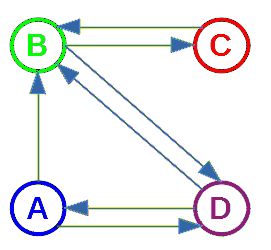
\includegraphics[width=1in]{quiz-on-individual-topics/pageranks.png}}
%\caption{\label{fig:pageranks} Four webpages with links.}
%\end{figure}



\end{document}

